%%%%%%%%%%%%%%%%%%%%%%%%%%%%%%%%%%%%%%%%%%%%%%%%%%%%%%%%%%%%%%%%%%%%%%
% Lớp 11 | Đường thẳng, mặt phẳng. Quan hệ song song trong | Phép chiếu song song
% Dạng 1H4?6-1: Câu hỏi lý thuyết
% Số câu: 44  (sinh tự động bởi tach_cau.py; từ nay thầy sửa trực tiếp file này)
%%%%%%%%%%%%%%%%%%%%%%%%%%%%%%%%%%%%%%%%%%%%%%%%%%%%%%%%%%%%%%%%%%%%%%

%%%%%%%%%%%%%%%% TRẮC NGHIỆM 4 PHƯƠNG ÁN %%%%%%%%%%%%%%%%

% nguồn: Ok_Toan11_TracNghiem_Lan2
\begin{ex}%[1H4N6-1]%[ma:0bc8f4f0]
	Cho hình lăng trụ $ABC.A'B'C'$, qua phép chiếu song song đường thẳng $CC'$, mặt phẳng  chiếu $(A'B'C')$ biến $M$ thành $M'$, trong đó $M$ là trung điểm của $BC$. Chọn mệnh đề \textbf{đúng}?
	\choice 
		{$M'$ là trung điểm của  $A'B'$}
		{\True $M'$ là trung điểm của  $B'C'$}
		{$M'$ là trung  điểm của $A'C'$}
		{$M'$ là  trọng tâm tam giác $A'B'C'$}
	 \loigiai{
		Ta có phép chiếu song song đường thẳng $CC'$ biến $C$ thành  $C'$, biến $B$ thành $B'$.\\
		Do $M$ là trung điểm của $BC$, suy ra $M'$  là trung điểm của $B'C'$.
	 }
\end{ex}

% nguồn: Ok_Toan11_TracNghiem_Lan2
\begin{ex}%[1H4N6-1]%[ma:c99af5c5]
	Qua phép chiếu song song, tính chất nào không  được bảo toàn?
	\choice 
		{\True Chéo nhau} 
		{Đồng quy} 
		{Song song} 
		 {Thẳng hàng}
	 \loigiai{
		Qua phép chiếu song song ảnh của hai đường thẳng cùng thuộc một  mặt phẳng.\\
		Suy ra tính chất chéo nhau  không được bảo toàn.
	 }
\end{ex}

% nguồn: Ok_Toan11_TracNghiem_Lan2
\begin{ex}%[1H4N6-1]%[ma:ad028fc6]
	Trong các mệnh đề sau, mệnh đề nào \textbf{sai}? 
	\choice 
		{Phép chiếu song song biến đường thẳng thành đường thẳng, biến tia thành tia,  biến đoạn thẳng thành đoạn thẳng}
		{\True Phép chiếu song song biến  hai đường thẳng song song thành hai đường thẳng song song}
		{Phép chiếu song song biến ba điểm thẳng hàng  thành ba điểm thẳng hàng và không thay đổi thứ tự của ba điểm đó}
		{Phép chiếu song song không làm thay đổi tỉ số độ dài của hai đoạn thẳng  nằm trên hai đường thẳng song song hoặc cùng nằm trên một mặt phẳng}
	\loigiai{ 
		Tính chất của phép chiếu song song: Phép chiếu song song biến hai đường thẳng song song thành hai đường  thẳng song song hoặc trùng nhau.\\
	Suy ra  B sai: Chúng có thể trùng nhau.}
\end{ex}

% nguồn: Ok_Toan11_TracNghiem_Lan2
\begin{ex}%[1H4N6-1]%[ma:0cd5e00a]
	Khẳng định nào sau đây \textbf{đúng}? 
	 \choice
		{\True Hình chiếu song song của một hình chóp  cụt có thể là một hình tam giác}
		{Hình chiếu song song của một hình chóp cụt có  thể là một đoạn thẳng}
		{Hình chiếu song song của một hình chóp cụt có  thể là một hình chóp cụt}
		{Hình chiếu song song của một hình chóp cụt  có thể là một điểm}
	\loigiai{ 
		Khẳng định đúng là \lq\lq Hình chiếu song song của một hình chóp cụt có thể là một hình tam  giác\rq\rq.
	 }
\end{ex}

% nguồn: Ok_Toan11_TracNghiem_Lan2
\begin{ex}%[1H4N6-1]%[ma:5bce25ab]
	Qua  phép chiếu song song, tính chất nào \textbf{không} được bảo toàn?
	 \choice
		{\True  Chéo nhau}
		 {Đồng qui}
		 {Song song}
		{Thẳng hàng} 
	\loigiai{ 
		Do  hai đường thẳng qua phép chiếu song song ảnh của chúng sẽ cùng thuộc một mặt phẳng, nên suy ra tính chất chéo nhau không được bảo toàn.
	} 
\end{ex}

% nguồn: Ok_Toan11_TracNghiem_Lan2
\begin{ex}%[1H4N6-1]%[ma:f013add9]
	Trong các mệnh đề sau mệnh đề  nào \textbf{sai}?
	 \choice
		 {Hình chiếu song song của hai đường thẳng chéo nhau có thể song song với nhau}
		{Một đường thẳng  có thể trùng với hình chiếu của nó}
		{\True Hình chiếu song  song của hai đường thẳng chéo nhau có thể trùng nhau}
		{Một tam giác bất kỳ đều có thể xem là hình biểu diễn  của một tam giác cân}
	 \loigiai{
		Mệnh đề sai là \lq\lq Hình chiếu song song của hai đường thẳng chéo nhau có thể trùng nhau\rq\rq, vì hình chiếu của  chúng chỉ có thể song song hoặc cắt nhau.
	} 
\end{ex}

% nguồn: Ok_Toan11_TracNghiem_Lan2
\begin{ex}%[1H4N6-1]%[ma:b6e10b83]
	Trong các mệnh đề  sau mệnh đề nào sai?
	 \choice
		{\True Một đường thẳng luôn  cắt hình chiếu của nó}
		{Một tam giác bất kỳ đề  có thể xem là hình biểu diễn của một tam giác cân}
		{Một đường thẳng có thể song song với hình chiếu của nó} 
		{Hình chiếu song song của  hai đường thẳng chéo nhau có thể song song với nhau}
	\loigiai{ 
		Mệnh đề sai là \lq\lq Một đường thẳng luôn  cắt hình chiếu của nó\rq\rq.
	 }
\end{ex}

% nguồn: Ok_Toan11_TracNghiem_Lan2
\begin{ex}%[1H4N6-1]%[ma:73e6d27a]
	Qua phép chiếu  song song biến ba đường thẳng song song thành
	\choice 
		{Ba đường thẳng đôi một song song  với nhau}
		{Một đường thẳng} 
		{Hai  đường thẳng song song}
		 {\True Cả ba trường hợp trên}
	\loigiai{ 
		Theo  tính chất của phép chiếu song song, ta thấy qua phép chiếu song song biến ba đường thẳng song song thành một đường thẳng, hoặc hai đường thẳng song song, hoặc ba đường thẳng đôi một song song với nhau.
	 }
\end{ex}

% nguồn: Ok_Toan11_TracNghiem_Lan2
\begin{ex}%[1H4N6-1]%[ma:f97829b7]
	Khẳng định nào sau  đây \textbf{sai}?
	\choice 
		{Phép chiếu song song  có thể biến đường tròn thành đường elip}
		{\True Phép chiếu song song  có thể biến đường tròn thành một điểm}
		{Phép chiếu song  song có thể biến đường tròn thành đoạn thẳng}
		{Phép chiếu song song có thể biến đường tròn thành đường  tròn}
	\loigiai{\begin{itemize}
		\item Phương chiếu vuông  góc với mặt phẳng chứa đường tròn biến đường tròn thành đường tròn.
		\item Phương chiếu nằm trong mặt phẳng chứa đường  tròn biến đường tròn thành đoạn thẳng.
		\item Phương chiếu cắt với  mặt phẳng chứa đường tròn biến đường tròn thành đường elip.
\end{itemize}}
\end{ex}

% nguồn: Ok_Toan11_TracNghiem_Lan2
\begin{ex}%[1H4N6-1]%[ma:5273dc65]
	Trong các mệnh  đề sau mệnh đề nào \textbf{sai}?
	\choice 
		 {Phép chiếu song song biến đường thẳng thành đường thẳng, biến tia thành tia, biến đoạn thẳng thành đoạn thẳng}
		 {\True Phép chiếu song song biến hai đường thẳng song song thành hai đường thẳng song song}
		{Phép chiếu song song biến ba điểm thẳng hàng thành ba điểm thẳng hàng và không thay đổi thứ tự của ba điểm  đó}
		{Phép chiếu song song không làm thay đổi tỉ số độ dài của hai đoạn thẳng nằm trên hai đường thẳng song song hoặc cùng nằm  trên một đường thẳng}
	 \loigiai{
		Tính chất  của phép chiếu song song: Phép chiếu song song biến hai đường thẳng song song thành hai đường thẳng song song hoặc trùng nhau.\\
		Suy ra mệnh đề sai là \lq\lq Phép chiếu song song biến hai  đường thẳng song song thành hai đường thẳng song song\rq\rq.
	 }
\end{ex}

% nguồn: Ok_Toan11_TracNghiem_Lan2
\begin{ex}%[1H4N6-1]%[ma:81fb891a]
	Hình chiếu song song của hai đường  thẳng chéo nhau không thể có vị trí nào trong các vị trí tương đối sau?
	 \choice
		 {Cắt nhau}
		{\True Chéo nhau} 
		 {Song song}
		 {Trùng nhau}
	\loigiai{Do hình chiếu của hai đường thẳng ban đầu nằm trên cùng một mặt  phẳng nên chúng không thể chéo nhau.}
\end{ex}

% nguồn: Ok_Toan11_TracNghiem_Lan2
\begin{ex}%[1H4N6-1]%[ma:8413eca4]
	 Phép chiếu song song biến hai đường thẳng song song thành
	\choice 
		{hai đường thẳng song song} 
		{hai  đường thẳng trùng nhau}
		{\True hai đường thẳng song  song hoặc trùng nhau}
		{hai đường thẳng chéo nhau} 
	 \loigiai{
	Phép chiếu song song biến hai đường thẳng song song thành hai đường  thẳng song song hoặc trùng nhau.}
\end{ex}

% nguồn: Ok_Toan11_TracNghiem_Lan2
\begin{ex}%[1H4N6-1]%[ma:d644774b]
	Hình  chiếu của hình vuông \textbf{không thể} là hình nào trong các hình sau?
	 \choice
		{Hình vuông} 
		{Hình  bình hành}
		{\True Hình thang} 
		{Hình  thoi}
	\loigiai{ 
		Theo tính chất của phép chiếu song  song và từ các phương án đã cho, ta thấy hình chiếu của hình vuông không thể là hình thang.
	} 
\end{ex}

% nguồn: Ok_Toan11_TracNghiem_Lan2
\begin{ex}%[1H4N6-1]%[ma:7f86ff9e]
	Trong các mệnh đề sau, mệnh  đề nào \textbf{sai}?
	 \choice
		{Phép chiếu song song bảo toàn thứ tự ba điểm thẳng  hàng}
		{\True  Phép chiếu song song không làm thay đổi tỉ số độ dài của hai đoạn thẳng}
		{Hình chiếu của hai đường  thẳng song song là hai đường thẳng song song hoặc trùng nhau}
		{Hình  chiếu song song của đường thẳng là đường thẳng}
	\loigiai{ Phép chiếu song song không làm thay đổi tỉ số  độ dài của hai đoạn thẳng khi hai đoạn thẳng đó nằm trên 2 đường thẳng song song hoặc nằm trên cùng một đường thẳng.
	} 
\end{ex}

% nguồn: Ok_TracNghiemLop11_Lan1
\begin{ex}%[1H4N6-1]%[ma:c4b5b178]
	Phép chiếu song song theo phương không song song với hoặc, mặt phẳng chiếu là, hai đường thẳng và biến thành và. Quan hệ  nào giữa và không được bảo toàn đối với phép chiếu song song?
	\choice 
		 {Cắt nhau}
		{\True Chéo nhau} 
		{Song song} 
		{Trùng  nhau}
	\loigiai{ 
	Phép chiếu song  song lên mặt phẳng không bảo toàn mối quan hệ giữa hai đường thẳng chéo nhau trong không gian.}
\end{ex}

% nguồn: Ok_TracNghiemLop11_Lan1
\begin{ex}%[1H4N6-1]%[ma:115ad7a6]
	Trong các mệnh đề sau, mệnh đề nào đúng? 
	 \choice
		{\True Hình chiếu song song của hai đường thẳng chéo nhau có thể song song với  nhau}
		{Hình chiếu song song của hai đường thẳng cắt nhau thì song song} 
		{Hình chiếu song song của một hình vuông  là một hình vuông}
		{Hình chiếu song song của một lục giác đều là  một lục giác đều}
	\loigiai{ 
	 }
\end{ex}

% nguồn: Ok_TracNghiemLop11_Lan1
\begin{ex}%[1H4N6-1]%[ma:f466b1ff]
	Cho các đoạn thẳng và đường thẳng không  song song hoặc không trùng với phương chiếu. Mệnh đề nào dưới đây là mệnh đề \textbf{sai}?
	 \choice
		{Phép chiếu song song biến  ba điểm thẳng hàng thành ba điểm thẳng hàng}
		{\True Phép chiếu song song không làm thay đổi tỉ số độ dài của hai đoạn thẳng} 
		{ Hình chiếu của hai  đường thẳng song song là hai đường thẳng song song hoặc trùng nhau}
		{Hình chiếu song song của một đường thẳng là một đường  thẳng}
	\loigiai{ 
	Mệnh đề \lq\lq Phép chiếu song song không làm thay đổi tỉ số độ dài của hai đoạn thẳng\rq\rq\, vì \lq\lq Phép chiếu song song không làm thay đổi tỉ số độ dài của hai đoạn thẳng cùng nằm trên một đường  thẳng hoặc nằm trên hai đường thẳng song song\rq\rq.}
\end{ex}

% nguồn: Ok_TracNghiemLop11_Lan1
\begin{ex}%[1H4N6-1]%[ma:220bee68]
	Cho tứ diện diện  $ABCD$. Gọi $M,N,K$ lần lượt là trung điểm của $AB$, $AD$, $MN$ và $L$ là một điểm nằm trên đoạn $BD$ sao cho $BL=\dfrac{1}{4}BD$.
	\choice 
		 {\True $KL\parallel AB$}
		{$KQ\parallel MC$} 
		 {$KL\parallel NC$}
		{$KQ\parallel  BC$}
	 \loigiai{
		\begin{center}
			\begin{tikzpicture}[scale=1,font=\footnotesize,line join=round,line cap=round,>=stealth]
					 \def\ac{4}
					\def\ab{3} 
					 \def\as{4}
					\def\gocA{40} 
					\coordinate[label=left:$A$]  (A) at (0,0);
					\coordinate[label=right:$C$] (C) at (\ac,0); 
					\coordinate[label=below left:$B$] (B) at  (-\gocA:\ab);
					\coordinate[label=above:$D$] (D)  at (70:\as);
					 \coordinate[label=below:$M$] (M) at ($(A)!.5!(B)$);
					\coordinate[label=left:$N$] (N) at ($(A)!.5!(D)$); 
					 \coordinate[label=left:$K$] (K) at ($(M)!.5!(N)$);
					\coordinate[label=right:$Q$] (Q)  at ($(B)!.5!(D)$);
					\coordinate[label=right:$L$] (L)  at ($(B)!.5!(Q)$);
					\draw  (A)--(B)--(C)--(D)--cycle (D)--(B)
						(K)--(L)--(M)--(N)--(Q)--(K); 
					 \draw[dashed] (A)--(C);
					\foreach \diem in {A,B,C,D,N,M,K,L,Q}\fill (\diem)  circle (1pt);
				\end{tikzpicture}
		\end{center}
		 Gọi $Q$ là trung điểm $BD$.\\
		 Qua phép chiếu song song theo phương $AB$ lên mặt phẳng $BCD$ biến:\\
		 $A$ thành $B$.\\
		$N$  thành $Q$.\\
		Vì  $BL=\dfrac{1}{4}BD=\dfrac{1}{2}BQ$ suy ra $L$ là trung điểm $BQ$.\\
		Do đó phép chiếu song song theo phương $AB$  lên $(BCD)$ biến $K$ thành $L$.\\
		Vậy $KL\parallel AB$. 
	 }
\end{ex}

% nguồn: Ok_TracNghiemLop11_Lan1
\begin{ex}%[1H4N6-1]%[ma:ffbf3b9c]
	Trong không gian, mệnh  đề nào sau đây đúng?
	\choice 
		{\True Phép chiếu song song biến hai đường thẳng cắt nhau thành hai đường thẳng cắt nhau  hoặc trùng nhau}
		{Phép chiếu song song biến  hai đường thẳng cắt nhau thành hai đường thẳng song song}
		{Phép chiếu song song biến hai đường thẳng cắt nhau thành  hai đường thẳng trùng nhau}
		{Phép chiếu song song biến hai đường thẳng cắt nhau thành hai đường thẳng  cắt nhau}
	 \loigiai{
	Theo tính chất của phép chiếu song song ta có phép chiếu song song biến hai đường thẳng  cắt nhau thành hai đường thẳng cắt nhau hoặc trùng nhau.}
\end{ex}

% nguồn: Ok_TracNghiemLop11_Lan1
\begin{ex}%[1H4N6-1]%[ma:3c581da2]
	Chọn tính chất đúng của phép chiếu  song song.
	\choice 
		{\True Phép chiếu song song giữ nguyên tỉ số độ dài của hai đoạn thẳng cùng nằm  trên một đường thẳng hoặc nằm trên hai đường thẳng song song}
		{Phép chiếu song song giữ nguyên tỉ số độ dài của hai đoạn thẳng  nằm trên đường thẳng song song}
		{Phép chiếu song song giữ nguyên độ dài của  đoạn thẳng}
		{Phép chiếu song song giữ nguyên tỉ  số độ dài của hai đoạn thẳng bất kì}
	 \loigiai{
	Tính chất đúng là phép chiếu song song giữ nguyên tỉ số độ dài của hai đoạn thẳng cùng nằm trên một đường  thẳng hoặc nằm trên hai đường thẳng song song.}
\end{ex}

% nguồn: Ok_TracNghiemLop11_Lan1
\begin{ex}%[1H4N6-1]%[ma:37fbc47b]
	Hình chiếu của hình  chữ nhật không thể là hình nào trong các hình sau?
	\choice 
		{\True Hình thang} 
		 {Hình bình hành}
		 {Hình chữ nhật}
		{Hình  thoi}
	\loigiai{ 
	Do phép chiếu song  song biến hai đường thẳng song song thành hai đường thẳng song song hoặc trùng nhau, nên không thể có Hình thang.}
\end{ex}

% nguồn: Ok_TracNghiemLop11_Lan1
\begin{ex}%[1H4N6-1]%[ma:af48123a]
	 Khẳng định nào sau đây \textbf{sai}?
	 \choice
		{Phép chiếu song song có thể  biến đường tròn thành đường tròn}
		{Phép chiếu song song có thể biến đường tròn thành đoạn  thẳng}
		{Phép chiếu song song có thể biến đường tròn thành đường  elip}
		{\True Phép chiếu song song có thể biến đường tròn thành một  điểm}
	\loigiai{ 
		Phương chiếu vuông góc với  mặt phẳng chứa đường tròn biến đường tròn thành đường tròn.\\
		 Phương chiếu nằm trong mặt phẳng chứa đường tròn biến đường tròn thành đoạn thẳng.\\
	Phương chiếu cắt (không vuông góc) với mặt phẳng chứa đường tròn  biến đường tròn thành đường elip}
\end{ex}

% nguồn: Ok_TracNghiemLop11_Lan1
\begin{ex}%[1H4N6-1]%[ma:2642686c]
	Cho tam giác $ABC$  ở trong mp $(\alpha)$ và phương $l$. Biết hình chiếu của tam giác $ABC$ lên mp $(P)$ là một đoạn thẳng. Khẳng định nào sau đây đúng ?
	\choice 
		{$(\alpha)\parallel (P)$} 
		 {$(\alpha)\equiv (P)$}
		{\True  $(\alpha)\parallel l$ hoặc $(\alpha)\supset l$}
		 {$A;B;C$ đều sai}
	\loigiai{ 
	Khi phương chiếu $l$ thỏa mãn $(\alpha)\parallel l$ hoặc $(\alpha)\supset l$ thì  các đoạn thẳng $AB$, $BC$, $CA$ có hình chiếu lên $(P)$ nằm trên giao tuyến của $(\alpha)$ và $(P)$.}
\end{ex}

% nguồn: Ok_TracNghiemLop11_Lan1
\begin{ex}%[1H4N6-1]%[ma:c656f05f]
	Hãy chọn câu trả lời đúng.  Trong không gian
	 \choice
		{Hình biểu diễn của một đoạn thẳng là một đoạn thẳng hoặc  một điểm}
		{\True Hình biểu diễn  của một hình tròn là một hình tròn}
		{Hình biểu diễn của một hình chữ nhật là một hình  chữ nhật hoặc một đoạn thẳng}
		{Hình biểu diễn của một góc  là một góc bằng nó}
	\loigiai{ 
	 }
\end{ex}

% nguồn: Ok_TracNghiemLop11_Lan1
\begin{ex}%[1H4N6-1]%[ma:ca7eaa69]
	Cho hình chóp $S.ABCD$ có đáy  là hình bình hành, gọi $M$ là trung điểm của $SC$.
	Hình chiếu song  song của điểm $M$ theo phương $AC$ lên mặt phẳng $(SAD)$ là điểm nào sau đây?
	 \choice
		 {Trung điểm của $SB$}
		{Trung điểm của $SD$} 
		 {Điểm $D$}
		{\True Trung điểm của  $SA$}
	\loigiai{ 
		\begin{center}
			\begin{tikzpicture}[scale=1,font=\footnotesize,line join=round,line cap=round,>=stealth]
					\def\bc{4} 
					\def\ba{2} 
					 \def\h{4}
					\def\gocB{30} 
					 \coordinate[label=below left:$B$] (B) at (0,0);
					\coordinate[label=above  left:$A$] (A) at (\gocB:\ba);
					\coordinate[label=below:$C$] (C) at  (\bc,0);
					 \coordinate[label=right:$D$] (D) at ($(C)-(B)+(A)$);
					\coordinate[label=above:$S$] (S) at  ($(A)+(0:.5)+(90:\h)$);
					\coordinate[label=right:$M$]  (M) at ($(S)!.5!(C)$);
					\coordinate[label=left:$N$] (N)  at ($(S)!.5!(A)$);
					 \draw (B)--(C)--(D)--(S)--cycle (S)--(C);
					\draw[dashed] (C)--(A)--(D) 
						(M)--(N) 
						 (S)--(A)--(B);
					\foreach \diem in {A,B,C,D,S,M,N}  \fill (\diem) circle (1pt);
					\newcommand{\gocv}[4][black]{\draw[#1]  ($(#3)!5pt!(#2)$)--($(#3)!2!($($(#3)!5pt!(#2)$)!.5!($(#3)!5pt!(#4)$)$)$)--($(#3)!5pt!(#4)$);}
				\end{tikzpicture}
		\end{center}
		Gọi $N$ là  trung điểm $SA$.\\
	Khi đó  $MN \parallel AC$ nên hình chiếu song song của điểm $M$ lên mặt phẳng $(SAD)$ là trung điểm $SA$.}
\end{ex}

% nguồn: Ok_TracNghiemLop11_Lan1
\begin{ex}%[1H4N6-1]%[ma:29be198e]
	 Trong không gian, mệnh đề nào sau đây đúng?
	 \choice
		{Phép chiếu song song biến hai đường thẳng cắt nhau thành hai đường  thẳng cắt nhau}
		{Phép chiếu song song biến hai đường thẳng  cắt nhau thành hai đường thẳng trùng nhau}
		{\True Phép chiếu song song biến hai đường thẳng cắt nhau thành hai đường  thẳng cắt nhau hoặc trùng nhau}
		{Phép chiếu song song biến  hai đường thẳng cắt nhau thành hai đường thẳng song song nhau}
	 \loigiai{
		Hai đường thẳng cắt nhau xác định  cho ta một mặt phẳng.\\
		Nếu phép chiếu song song với phương chiếu không song song với mặt  phẳng chứa hai đường thẳng cắt nhau thì cho ta hai đường thẳng cắt nhau.\\
	Nếu phép chiếu song song với  phương chiếu song song với mặt phẳng chứa hai đường thẳng cắt nhau thì cho ta môộ đường thẳng hay cho ta hai đường thẳng trùng nhau.}
\end{ex}

% nguồn: Ok_TracNghiemLop11_Lan1
\begin{ex}%[1H4N6-1]%[ma:b138e427]
	Hình vẽ nào sau đây $\textbf{không  phải}$ hình biểu diễn của hình chóp tứ giác $S.ABCD$?
	 \choice
		 {
		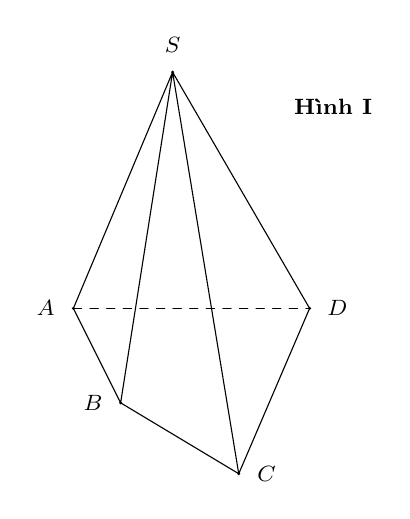
\begin{tikzpicture}[line join=round,line cap=round,>=stealth,scale=0.6,font=\footnotesize]
				\tikzset{every  node/.style={outer sep=-0.5mm}}
				\foreach \x/\y/\n in {0/0/A,5/0/D,1/-2/B,3.5/-3.5/C,2.1/5/S} \coordinate  (\n) at (\x,\y);
				\draw[dashed]  (A)--(D);
				\draw (A)--(S)--(B)--(C)--(S)--(D)--(C)--(B)--cycle; 
				\foreach  \t/\g in {A/180,B/180,C/0,D/0,S/90}{
					\fill (\t) circle (1pt)  node[shift={(\g:10pt)}]{$ \t $};}
				\draw (5.5,4) node[above]{\textbf{Hình I}}; 
			\end{tikzpicture}
		 }
		 {
		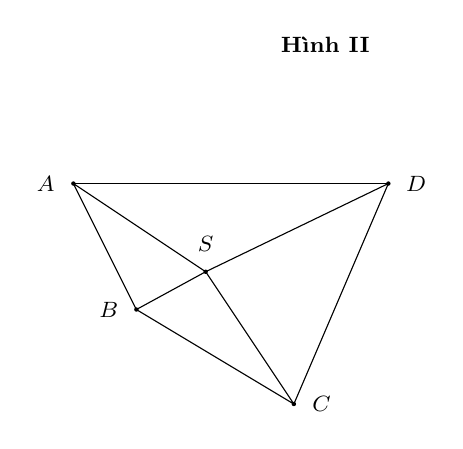
\begin{tikzpicture}[line join=round,line cap=round,>=stealth,scale=0.8,font=\footnotesize]
				\tikzset{every node/.style={outer sep=-0.5mm}} 
				\foreach \x/\y/\n in {0/0/A,5/0/D,1/-2/B,3.5/-3.5/C,2.1/-1.4/S} \coordinate  (\n) at (\x,\y);
				\draw  (A)--(D);
				\draw (A)--(S)--(B)--(C)--(S)--(D)--(C)--(B)--cycle; 
				\foreach \t/\g in  {A/180,B/180,C/0,D/0,S/90}{
					\fill (\t)  circle (1pt) node[shift={(\g:10pt)}]{$ \t $};}
				\draw (4,2) node[above]{\textbf{Hình II}}; 
			\end{tikzpicture}
		 }
		 {
		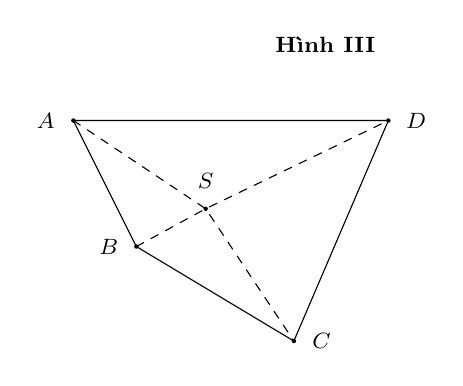
\begin{tikzpicture}[line join=round,line cap=round,>=stealth,scale=0.8,font=\footnotesize]
				\tikzset{every node/.style={outer  sep=-0.5mm}}
				\foreach \x/\y/\n  in {0/0/A,5/0/D,1/-2/B,3.5/-3.5/C,2.1/-1.4/S} \coordinate (\n) at (\x,\y);
				 \draw (A)--(D)--(C)--(B)--cycle;
				 \draw[dashed] (A)--(S)--(C)
					(B)--(S)--(D); 
				 \foreach \t/\g in {A/180,B/180,C/0,D/0,S/90}{
					\fill (\t) circle (1pt)  node[shift={(\g:10pt)}]{$ \t $};}
				\draw  (4,1) node[above]{\textbf{Hình III}};
			\end{tikzpicture}
		} 
		{\True 
		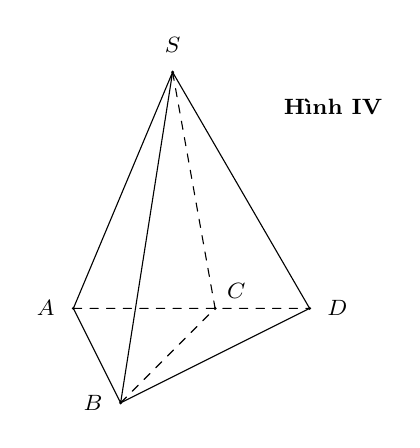
\begin{tikzpicture}[line join=round,line cap=round,>=stealth,scale=0.6,font=\footnotesize]
				\tikzset{every  node/.style={outer sep=-0.5mm}}
				\foreach \x/\y/\n in {0/0/A,5/0/D,1/-2/B,3/0/C,2.1/5/S} \coordinate (\n)  at (\x,\y);
				 \draw (S)--(A)--(B)--(S)--(D)--(B);
				\draw[dashed] (A)--(C)--(D) 
					(B)--(C)--(S); 
				\foreach \t/\g in {A/180,B/180,C/40,D/0,S/90}{ 
					\fill (\t) circle (1pt)  node[shift={(\g:10pt)}]{$ \t $};}
				\draw (5.5,4) node[above]{\textbf{Hình  IV}};
			\end{tikzpicture}
		} 
	\loigiai{ 
		$\textbf{Hình IV}$ có $3$ điểm $A$, $C$, $D$ thẳng hàng $\Rightarrow$ Phương chiếu phải song song với mặt phẳng $(ABC)$, tức là song song với mặt phẳng $(ABCD)$. Khi đó $4$ điểm $A$, $B$, $C$, $D$ phải  thẳng hàng $\Rightarrow$ $\textbf{Hình IV}$ sai.
	} 
\end{ex}

% nguồn: Ok_TracNghiemLop11_Lan1
\begin{ex}%[1H4N6-1]%[ma:d02ba149]
	Chọn mệnh đề  đúng trong các mệnh đề sau đây?
	 \choice
		{\True Trong  không gian hai đường thẳng chéo nhau thì không có điểm chung}
		{Trong không gian hai đường thẳng phân biệt cùng song song với một mặt phẳng  thì song song với nhau}
		{Nếu mặt phẳng $(P)$ chứa hai đường thẳng cùng song song với mặt phẳng $(Q)$ thì $(P)$ và $(Q)$ song song với nhau} 
		{Trong không  gian hình biểu diễn của một góc thì phải là một góc bằng nó}
	 \loigiai{
	Mệnh đề đúng là \lq\lq  Trong không gian hai đường thẳng chéo nhau thì không có điểm chung.\rq\rq}
\end{ex}

% nguồn: Ok_TracNghiemLop11_Lan1
\begin{ex}%[1H4N6-1]%[ma:51044dcf]
	Qua phép chiếu song song, tính chất nào không  được bảo toàn?
	 \choice
		 {\True Chéo nhau}
		{đồng  qui}
		 {Song song}
		 {thẳng hàng}
	 \loigiai{
	Qua phép chiếu song song,  tính chất chéo nhau không được bảo toàn}
\end{ex}

% nguồn: Ok_TracNghiemLop11_Lan1
\begin{ex}%[1H4N6-1]%[ma:a5735342]
	Khẳng định  nào sau đây \textbf{sai}?
	 \choice
		{\True Phép chiếu song song có thể biến một đường tròn thành một điểm} 
		{Phép chiếu song song có thể biến  một đường tròn thành một đoạn thẳng}
		{Phép chiếu song song có thể biến một  đường tròn thành một đường tròn}
		{Phép chiếu song song có thể biến một đường tròn thành  một elip}
	 \loigiai{
		Theo tính chất của phép chiếu song song ta có phương án \lq\lq{\it Phép chiếu song song có thể biến  một đường tròn thành một điểm}\rq\rq\, là phương án sai.
	} 
\end{ex}

% nguồn: Ok_TracNghiemLop11_Lan1
\begin{ex}%[1H4N6-1]%[ma:012e2184]
	Qua phép chiếu  song song lên mặt phẳng $(P)$, hai đường thẳng $a$ và $b$ có hình chiếu là hai đường thẳng song song $a’$ và $b’$. Khi đó
	 \choice
		{$a$ và $b$ phải song  song với nhau}
		 {$a$ và $b$ phải cắt nhau}
		{\True $a$ và $b$ có thể chéo nhau hoặc song song  với nhau}
		{$a$ và $b$ không thể song song} 
	 \loigiai{
		Nếu $a’  \parallel b’ $ suy ra mặt phẳng ($a$, $a’$) song song mặt phẳng ($b$, $b’$).\\
		Khi đó $a$  và $b$ có thể song song hoặc chéo nhau.
	} 
\end{ex}

% nguồn: Ok_TracNghiemLop11_Lan1
\begin{ex}%[1H4N6-1]%[ma:d48ed072]
	Xét phép chiếu song song lên mặt phẳng  $(P)$ theo phương $l$.Trong các mệnh đề sau mệnh đề nào đúng?
	\choice 
		{Hình chiếu song song của hai đường thẳng cắt nhau có thể song song  với nhau}
		{\True Hình chiếu song song của hai đường thẳng chéo  nhau có thể song song với nhau}
		{Hình chiếu  song song của hai đường thẳng chéo nhau thì song song với nhau}
		{Các mệnh  đề trên đều sai}
	 \loigiai{
	Hình chiếu song song của hai đường thẳng chéo nhau có thể song song với nhau; cũng có thể cắt nhau. Do đó mệnh đề đúng là Hình chiếu song  song của hai đường thẳng chéo nhau có thể song song với nhau}
\end{ex}

% nguồn: Ok_TracNghiemLop11_Lan1
\begin{ex}%[1H4N6-1]%[ma:44f74a7f]
	Mệnh đề nào sau đây  {\bf sai}?
	 \choice
		{Phép chiếu song song biến ba điểm thẳng hàng thành ba điểm  thẳng hàng và không làm thay đổi thứ tự ba điểm đó}
		{Phép chiếu song  song biến đoạn thẳng thành đoạn thẳng}
		 {Phép chiếu song song biến tia thành tia}
		{\True Phép chiếu song song biến hai đường thẳng song  song thành hai đường thẳng song song}
	 \loigiai{
	Mệnh đề \lq\lq Phép chiếu song song biến hai đường thẳng song song thành hai đường thẳng song  song\rq\rq\ sai vì phép chiếu song song biến hai đường thẳng song song thành hai đường thẳng song song hoặc trùng nhau.}
\end{ex}

% nguồn: Ok_TracNghiemLop11_Lan1
\begin{ex}%[1H4N6-1]%[ma:c9e432eb]
	Một tấm bảng nghiêng so với mặt đất được chiếu lên bức tường thẳng đứng bằng ánh sáng chiếu xiên  từ một nguồn sáng xa. Hình ảnh của tấm bảng trên bức tường sẽ là
	\choice 
		{Một đường thẳng} 
		 {Một hình tam giác}
		{\True Một hình chữ  nhật}
		{Một hình  tròn}
	 \loigiai{
		\begin{itemize}
			\item Khi ánh sáng chiếu xiên từ một nguồn sáng xa, các tia chiếu song song sẽ  chiếu hình ảnh của tấm bảng nghiêng lên bức tường thẳng đứng.
			\item Tấm bảng nghiêng có hình chữ nhật, khi chiếu song song lên bức tường, hình ảnh của nó vẫn giữ nguyên  dạng là hình chữ nhật, nhưng có thể bị biến dạng theo góc chiếu.
			\item Tuy nhiên, do tính chất của phép chiếu song song, các  cạnh của hình chữ nhật sẽ vẫn song song và duy trì hình dạng cơ bản của nó.
		\end{itemize}
		Vậy hình ảnh của tấm bảng trên  bức tường sẽ là \lq\lq Một hình chữ nhật\rq\rq.
	} 
\end{ex}

% nguồn: Ok_Toan11_TracNghiem_Lan2
\begin{ex}%[1H4H6-1]%[ma:411d17e7]
	Phép chiếu song song theo phương $l$ không song song với $a$ hoặc $b$, mặt phẳng chiếu là $(P)$, hai đường thẳng $a$ và $b$ biến thành $a'$  và $b'$. Quan hệ nào giữa $a$ và $b$ không được bảo toàn trong phép chiếu song song?
	 \choice
		 {Cắt nhau}
		{Trùng nhau} 
		{Song song} 
		{\True  Chéo nhau}
	 \loigiai{
		Do $a'$ và $b'$ cùng được chứa trong mặt phẳng chiếu  $(P)$, suy ra tính chất chéo nhau không được bảo toàn.
	} 
\end{ex}

% nguồn: Ok_Toan11_TracNghiem_Lan2
\begin{ex}%[1H4H6-1]%[ma:12195af9]
	Cho tam giác $ABC$ ở trong mặt phẳng $(\alpha)$ và phương $\ell$. Biết hình chiếu của tam giác $ABC$ lên mặt phẳng $(P)$  là một đoạn thẳng. Khẳng định nào sau đây \textbf{đúng}?
	 \choice
		{$(\alpha)\parallel  (P)$}
		{$(\alpha)\equiv  (P)$}
		{\True $(\alpha)\parallel  \ell$ hoặc $(\alpha)\supset \ell$}
		{$(\alpha)\parallel \ell$} 
	 \loigiai{
		Khi phương chiếu $\ell$ song song hoặc được chứa trong mặt phẳng $\alpha$ thì hình chiếu của tam giác là đoạn thẳng trên mặt  phẳng $(P)$.
	 }
\end{ex}

% nguồn: Ok_Toan11_TracNghiem_Lan2
\begin{ex}%[1H4H6-1]%[ma:755c1ef1]
	 Khẳng định nào sau đây đúng?
	\choice 
		{Hình chiếu song song của hình lập  phương $ABCD.A'B'C'D'$ theo phương $AA'$ lên mặt phẳng $(ABCD)$ là hình bình hành}
		{\True Hình chiếu song song của hình lập phương $ABCD.A'B'C'D'$ theo phương $AA'$ lên mặt phẳng $(ABCD)$ là hình vuông} 
		{Hình chiếu song song của hình lập phương $ABCD.A'B'C'D'$ theo phương $AA'$ lên mặt phẳng $(ABCD)$ là hình  thoi}
		{Hình chiếu song song của  hình lập phương $ABCD.A'B'C'D'$ theo phương $AA'$ lên mặt phẳng $(ABCD)$ là một tam giác}
	\loigiai{ 
		Qua phép chiếu song song đường  thẳng $AA'$ lên mặt phẳng $(ABCD)$ sẽ biến $A'$ thành $A$, biến $B'$ thành $B$, biến $C'$ thành $C$, biến $D'$ thành $D$.\\
		Nên hình chiếu  song song của hình lập phương $ABCD.A'B'C'D'$ theo phương $AA'$ lên mặt phẳng $(ABCD)$ là hình vuông.
	} 
\end{ex}

% nguồn: Ok_TracNghiemLop11_Lan1
\begin{ex}%[1H4H6-1]%[ma:bf59a1d8]
	Trong không gian, khẳng  định nào sau đây đúng?
	 \choice
		{Phép chiếu song song luôn biến hai đường  thẳng song song thành hai đường thẳng song song}
		 {Hình chiếu song song của một đường thẳng là một đường thẳng}
		{\True Hình  biểu diễn của một hình tròn qua phép chiếu song song có thể là một hình elip}
		{Phép chiếu song song  biến ba điểm thẳng hàng thành ba điểm thẳng hàng và không làm thay đổi thứ tự ba điểm đó}
	\loigiai{ 
		\begin{itemize}
			\item Phương chiếu song song với $(a, b)$ với $a\parallel b$ thì ảnh  là hai đường thẳng trùng nhau.
			\item Phương chiếu song song với đường thẳng thì hình chiếu  là một điểm.
			\item Phương chiếu tạo với mặt  phẳng chứa đường tròn một góc nhọn thì được một hình elip.
			\item Phương chiếu song song với đường thẳng chứa ba điểm thì  ảnh là ba điểm trùng nhau (một điểm).
		\end{itemize}
	 }
\end{ex}

% nguồn: Ok_TracNghiemLop11_Lan1
\begin{ex}%[1H4H6-1]%[ma:4477e23a]
	Cho hình hộp $ABCD.A'B'C'D'$. Gọi $M$, $M'$ lần lượt là trung điểm của các cạnh $BC$, $B'C'$. Hình chiếu của $\triangle B'DM$ qua phép chiếu  song song trên $(A'B'C'D')$ theo phương $AA'$ là
	\choice 
		{$\triangle  B'A'M'$}
		 {$\triangle C'D'M'$}
		{$\triangle  DMM'$}
		{\True $\triangle B'D'M'$} 
	 \loigiai{
	\immini{Phép chiếu song song theo phương $AA'$ biến $B'$ thành chính nó, biến $D$ thành $D'$, biến $M$ thành $M'$ do đó biến $\triangle B'DM$ thành $\triangle B'D'M'$.}{\begin{tikzpicture}[scale=1,font=\footnotesize,line join = round,line cap = round,>= stealth]
		 \coordinate (A) at (0,0);
		 \def\x{3}
		 \def\y{2}
		 \def\z{3}
		\def\g{30} 
		\def\n{85} 
		\coordinate (B)  at ($(A)+(\x,0)$);
		\coordinate (D) at ($(A)+(\g:\y)$); 
		\coordinate  (C) at ($(B)+(D)-(A)$);
		\coordinate (A')  at ($(A)+(\n:\z)$);
		\coordinate (B')  at ($(B)+(\n:\z)$);
		\coordinate (C')  at ($(C)+(\n:\z)$);
		\coordinate (D') at ($(D)+(\n:\z)$); 
		\coordinate (M) at  ($(B)!.5!(C)$);
		\coordinate (M') at  ($(B')!.5!(C')$);
		\draw  (A)--(B)--(B')--(A')--cycle;
		\draw  (A')--(D')--(C')--(B');
		 \draw (B)--(C)--(C');
		\draw[dashed] (A)--(D)--(D') 
			 (D)--(C);
		 \draw[dashed] (B')--(D)--(M);
		\draw[]  (B')--(M)--(M');
		\foreach \p/\g  in {A/180,B/-45,C/-45,D/-90,A'/90,B'/100,C'/90,D'/90,M/-10,M'/100} \draw[blue,fill=white] (\p) circle (.5pt) node [shift={(\g:.3)}] {$\p$};
	\end{tikzpicture}
		 }
	 }
\end{ex}


%%%%%%%%%%%%%%%% ĐÚNG/SAI %%%%%%%%%%%%%%%%

% nguồn: Ok_dungsai_lop11_Lan2
\begin{ex}%[1H4N6-1]%[ma:cf891332]
	Xét tính đúng sai của  các mệnh đề sau:
	 \choiceTF
		{\True Phép chiếu song song biến đường thẳng thành đường thẳng,  biến tia thành tia, biến đoạn thẳng thành đoạn thẳng}
		{Phép chiếu song song biến hai  đường thẳng song song thành hai đường thẳng song song}
		{\True Phép chiếu song song biến ba điểm thẳng hàng thành ba điểm thẳng hàng và không thay đổi thứ tự của ba điểm  đó}
		{\True Phép chiếu song song không làm thay đổi tỉ số độ dài của hai  đoạn thẳng nằm trên hai đường thẳng song song hoặc cùng nằm trên một đường thẳng}
	\loigiai{ 
		Theo tính chất của phép chiếu  song song.
		\begin{itemchoice}
			\itemch \textbf{Đúng.} 
			\itemch \textbf{Sai.}\\ 
			Vì phép chiếu song song biến hai đường thẳng song song thành hai đường thẳng song song  hoặc trùng nhau.
			\itemch  \textbf{Đúng.}
			 \itemch \textbf{Đúng.}
		\end{itemchoice}
	 }
\end{ex}

% nguồn: Ok_dungsai_lop11_Lan2
\begin{ex}%[1H4N6-1]%[ma:f40c01d1]
	Cho các  đoạn thẳng và đường thẳng không song song hoặc không trùng với phương chiếu.
	\choiceTF 
		{\True Phép chiếu song song bảo toàn thứ tự ba điểm thẳng hàng} 
		{Phép chiếu song song không làm thay đổi tỉ  số độ dài của hai đoạn thẳng}
		{\True Hình chiếu của hai đường  thẳng song song là hai đường thẳng song song hoặc trùng nhau}
		{\True Hình chiếu song  song của một đường thẳng là một đường thẳng}
	\loigiai{ 
		\begin{itemchoice}
			\itemch Phép chiếu song  song bảo toàn thứ tự ba điểm thẳng hàng.
			\itemch Phát biểu đúng là \lq\lq Phép chiếu song song không làm thay đổi tỉ số độ dài của hai đoạn thẳng cùng nằm trên một đường thẳng hoặc nằm trên hai đường thẳng song song\rq\rq. 
			\itemch Hình  chiếu của hai đường thẳng song song là hai đường thẳng song song hoặc trùng nhau.
			\itemch Hình chiếu song song của một đường thẳng là một  đường thẳng.
		\end{itemchoice}
	 }
\end{ex}

% nguồn: Ok_dungsai_lop11_Lan2
\begin{ex}%[1H4H6-1]%[ma:05170320]
	 Xét tính đúng sai của các mệnh đề sau:
	\choiceTF 
		{Một đường thẳng luôn cắt hình  chiếu của nó}
		{\True Một tam giác bất  kỳ đề có thể xem là hình biểu diễn của một tam giác cân}
		{Một đường thẳng không thể song song với hình chiếu của  nó}
		{\True Hình chiếu song song của hai  đường thẳng chéo nhau có thể song song với nhau}
	\loigiai{ 
		\begin{itemchoice}
			\itemch  \textbf{Sai.}\\
			Vì hình chiếu của một  đường thẳng có thể là một đường thẳng song song với nó.
			\itemch  \textbf{Đúng.}
			\itemch \textbf{Sai.}\\ 
			Vì hình chiếu của một đường thẳng là một đường thẳng song song với nó khi  đường thẳng ban đầu song song với mặt phẳng chiếu.
			\itemch  \textbf{Đúng.}\\
			Tuỳ vào phương chiếu thì có thể. 
		\end{itemchoice}
	} 
\end{ex}

% nguồn: Ok_dungsai_lop11_Lan2
\begin{ex}%[1H4H6-1]%[ma:c3b935bb]
	Xét tính đúng sai của các mệnh đề sau: 
	 \choiceTF
		{\True Hình chiếu song song của một  hình chóp cụt có thể là một hình tam giác}
		{Hình chiếu song song của  một hình chóp cụt có thể là một đoạn thẳng}
		{Hình chiếu song song của một hình chóp cụt có thể là một hình chóp  cụt}
		{Hình chiếu song song  của một hình chóp cụt có thể là một điểm}
	 \loigiai{
		Qua phép chiếu song song chỉ có thể biến  hình chóp cụt thành một đa giác.
		\begin{itemchoice}
			 \itemch \textbf{Đúng.}
			 \itemch \textbf{Sai.}\\
			Vì phép chiếu song song biến  hai đường thẳng song song thành hai đường thẳng song song hoặc trùng nhau.
			\itemch  \textbf{Sai.}
			\itemch  \textbf{Sai.}
		\end{itemchoice}
	 }
\end{ex}

% nguồn: Ok_dungsai_lop11_Lan2
\begin{ex}%[1H4H6-1]%[ma:4cba2494]
	Cho các đoạn thẳng và đường thẳng \textbf{không} song song hoặc \textbf{không} trùng với phương chiếu. Khi  đó
	\choiceTF 
		{\True Phép chiếu song song bảo toàn thứ tự ba  điểm thẳng hàng}
		{Phép chiếu song song \textbf{không} làm thay đổi tỉ số độ dài của hai đoạn thẳng} 
		{\True Hình chiếu  của hai đường thẳng song song là hai đường thẳng song song hoặc trùng nhau}
		{\True Hình chiếu song song của một đường thẳng là một đường  thẳng}
	\loigiai{ 
		\begin{itemchoice}
			 \itemch \textbf{Đúng.}
			\itemch  \textbf{Sai.}\\
			Phép chiếu song song \textbf{không} làm thay đổi tỉ số độ dài của hai đoạn thẳng cùng nằm trên một đường thẳng hoặc nằm trên hai đường thẳng  song song.
			 \itemch \textbf{Đúng.}
			\itemch \textbf{Đúng.} 
		\end{itemchoice}
	} 
\end{ex}
